%!TEX root = ../thesis.tex
\chapter{Experimental Results\label{ch:experiment}}

We used the 3D palmprint acquisition device developed in ~\cite{Zhang:2009dp} to establish a 3D palmprint database containing 8000 samples collected from 400 palms. The 3D palmprint samples were collected in two separated sessions, 10 samples in each session. The average time interval between the two sessions is one month. The collection procedure required volunteers to put their palms naturally and without force on the device. As mentioned in Section ~\ref{sec:methodology:roiextraction}, the original spatial resolution of the data was 768$\times$576. After ROI extraction, the central part (400$\times$400) was extracted and down-sampled to (200$\times$200) for feature extraction and recognition.

%!TEX root = chapter-experiment.tex
\section{Optimizing Parameters}
\label{sec:experiment:parameters}

The database was divided into a training part (the first session of 4000 samples) and a testing part (the second session of 4000 samples). As described in Section ~\ref{ssec:methodology:lda}, the dimension of the proposed  features is $1+N+N\times M$. To select the value of $M$ and $N$, a series of verifications on the training database were carried out where the class of the input palmprint was known. Each of the 3D samples was matched with the remaining samples in the training database. A successful match is where the two samples are from the same class. This is referred to as intra-class matching and the candidate image is said to be genuine. An unsuccessful match is referred to as inter-class matching and the candidate image is said to be an impostor. Treating the features as a point in the $1+N+N\times M$ dimension space, Euclidian distance is used as the matching score.


%!TEX root = chapter-experiment.tex
\section{Optimizing Parameters}
\label{sec:experiment:parameters}

The database was divided into a training part (the first session of 4000 samples) and a testing part (the second session of 4000 samples). As described in Section ~\ref{ssec:methodology:lda}, the dimension of the proposed  features is $1+N+N\times M$. To select the value of $M$ and $N$, a series of verifications on the training database were carried out where the class of the input palmprint was known. Each of the 3D samples was matched with the remaining samples in the training database. A successful match is where the two samples are from the same class. This is referred to as intra-class matching and the candidate image is said to be genuine. An unsuccessful match is referred to as inter-class matching and the candidate image is said to be an impostor. Treating the features as a point in the $1+N+N\times M$ dimension space, Euclidian distance is used as the matching score.


%!TEX root = chapter-experiment.tex
\section{Optimizing Parameters}
\label{sec:experiment:parameters}

The database was divided into a training part (the first session of 4000 samples) and a testing part (the second session of 4000 samples). As described in Section ~\ref{ssec:methodology:lda}, the dimension of the proposed  features is $1+N+N\times M$. To select the value of $M$ and $N$, a series of verifications on the training database were carried out where the class of the input palmprint was known. Each of the 3D samples was matched with the remaining samples in the training database. A successful match is where the two samples are from the same class. This is referred to as intra-class matching and the candidate image is said to be genuine. An unsuccessful match is referred to as inter-class matching and the candidate image is said to be an impostor. Treating the features as a point in the $1+N+N\times M$ dimension space, Euclidian distance is used as the matching score.


\input{ch-experiment/tables/parameters}

Table ~\ref{tab:experiment:parameters} shows the Equal Error Rate (EER) for $N=4,8,16$ and $M=8,16,32,64$. The best result, as adopted in Chapter ~\ref{ch:methodology}, is $N=8$ and $M=32$.


In order to balance accuracy and efficiency, we chose $N=8$ and $M=32$ in the following experiments. This means the features have $1+N+N\times M=265$ dimensions.

\input{ch-experiment/tables/verification}

Table ~\ref{tab:experiment:verification} shows the verification results by MD, HCA, RLL and their combined results. From the last column of Table ~\ref{tab:experiment:verification} we can see using the combined three features will achieve a lower EER than each of the individual features.

As described in Section ~\ref{ssec:methodology:lda}, we use the OLDA method to reduce features to a lower dimension $\Gamma$. To decide the optimal value of $\Gamma$, we carried out a series of recognition experiments on the 4000 sample training database. We divided this database into two equal parts and then chose the first five samples of every palm for training and set aside the rest for testing. As shown in Section ~\ref{ssec:methodology:lda}, $\Gamma$ is equal to q in (13). Instead of setting $q=rank(B)$, we set $q=1,2,\dots,10,12,15,20,30$.

\input{ch-experiment/tables/gamma}

Table ~\ref{tab:experiment:gamma} shows the recognition results.

\begin{figure}[htb]
  \begin{center}
    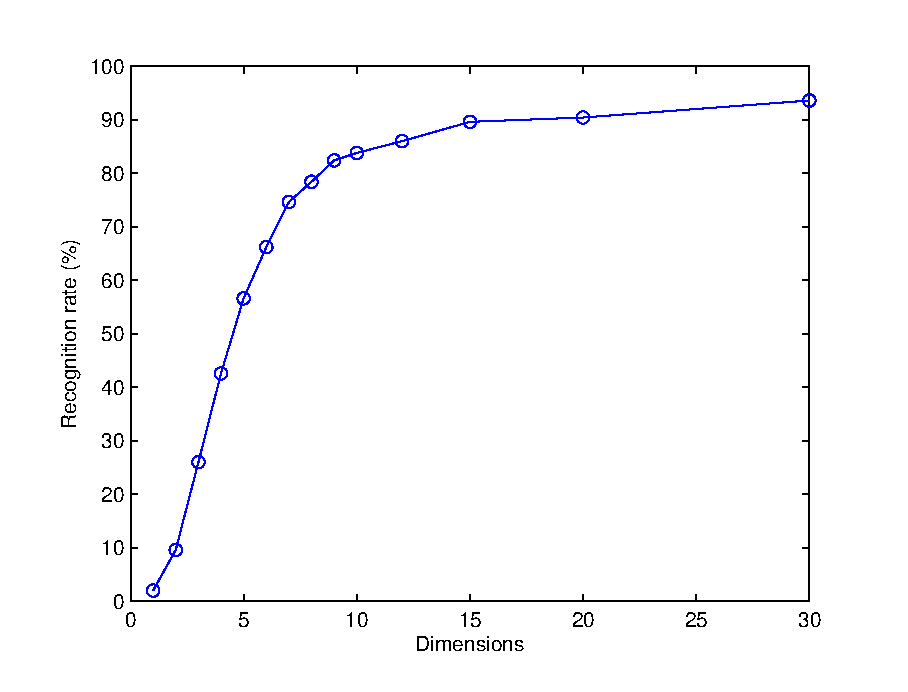
\includegraphics[width=\linewidth]{ch-experiment/figures/gamma}
    \caption[Recognition rate by OLDA for different dimensions]{Recognition rate by OLDA for different dimensions}
    \label{fig:experiment:gamma}
  \end{center}
\end{figure}

According to the curve shown in Figure ~\ref{fig:experiment:gamma}, $\Gamma=15$ is a good choice for the following experiments with balanced recognition rate and computation.

Table ~\ref{tab:experiment:parameters} shows the Equal Error Rate (EER) for $N=4,8,16$ and $M=8,16,32,64$. The best result, as adopted in Chapter ~\ref{ch:methodology}, is $N=8$ and $M=32$.


In order to balance accuracy and efficiency, we chose $N=8$ and $M=32$ in the following experiments. This means the features have $1+N+N\times M=265$ dimensions.

% Table generated by Excel2LaTeX from sheet 'Sheet2'
\begin{table}[htbp]
  \centering
  \caption{The EER of 3D palmprint verification for with each feature and the combined feature}
    \begin{tabular}{ccccc}
    \toprule
    Global features & MD    & HCA   & RLL   & MD+HCA+RLL \\
    \midrule
    EER(\%) & 25.8  & 20.4  & 18.6  & 12.32 \\
    \bottomrule
    \end{tabular}%
  \label{tab:experiment:verification}%
\end{table}%


Table ~\ref{tab:experiment:verification} shows the verification results by MD, HCA, RLL and their combined results. From the last column of Table ~\ref{tab:experiment:verification} we can see using the combined three features will achieve a lower EER than each of the individual features.

As described in Section ~\ref{ssec:methodology:lda}, we use the OLDA method to reduce features to a lower dimension $\Gamma$. To decide the optimal value of $\Gamma$, we carried out a series of recognition experiments on the 4000 sample training database. We divided this database into two equal parts and then chose the first five samples of every palm for training and set aside the rest for testing. As shown in Section ~\ref{ssec:methodology:lda}, $\Gamma$ is equal to q in (13). Instead of setting $q=rank(B)$, we set $q=1,2,\dots,10,12,15,20,30$.

% Table generated by Excel2LaTeX from sheet 'Sheet3'
\begin{table}[htbp]
  \centering
  \caption{Recognition rate by OLDA for different dimensions}
    \tabcolsep=0.11cm
    \begin{tabular}{|r|c|c|c|c|c|c|c|c|c|c|c|c|c|c|}
    \hline
        $\Gamma$  & 1     & 2     & 3     & 4     & 5     & 6     & 7     & 8     & 9     & 10    & 12    & 15    & 20    & 30 \\
    \hline
    Recognition rate (\%) & {2} & {9.6} & {26} & {42.6} & {56.6} & {66.2} & {74.6} & {78.4} & {82.4} & {83.8} & {86} & {89.6} & {90.4} & {93.6} \\
	\hline
    \end{tabular}%
  \label{tab:experiment:gamma}%
\end{table}%


Table ~\ref{tab:experiment:gamma} shows the recognition results.

\begin{figure}[htb]
  \begin{center}
    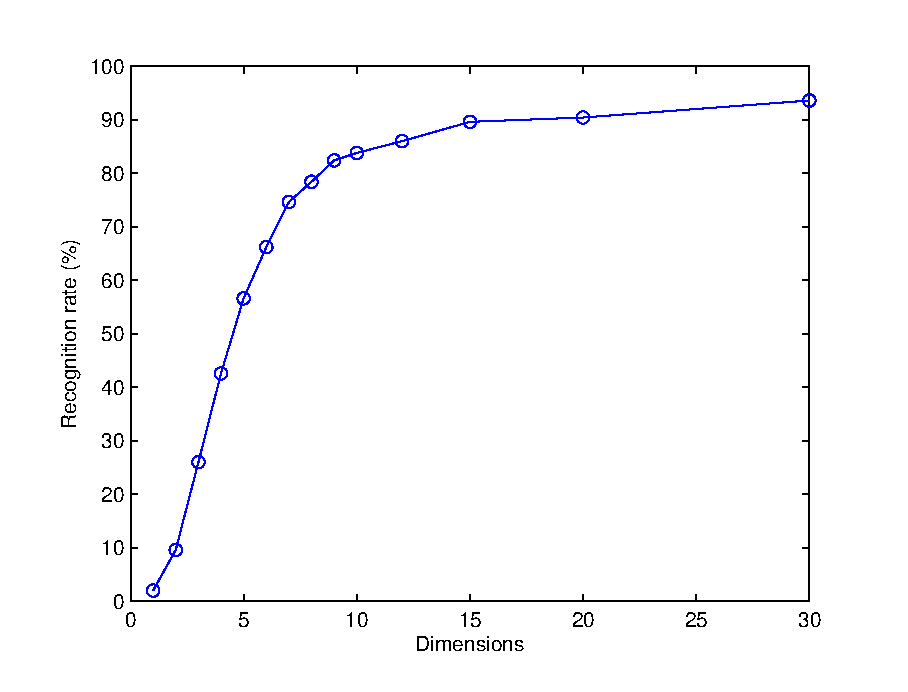
\includegraphics[width=\linewidth]{ch-experiment/figures/gamma}
    \caption[Recognition rate by OLDA for different dimensions]{Recognition rate by OLDA for different dimensions}
    \label{fig:experiment:gamma}
  \end{center}
\end{figure}

According to the curve shown in Figure ~\ref{fig:experiment:gamma}, $\Gamma=15$ is a good choice for the following experiments with balanced recognition rate and computation.

Table ~\ref{tab:experiment:parameters} shows the Equal Error Rate (EER) for $N=4,8,16$ and $M=8,16,32,64$. The best result, as adopted in Chapter ~\ref{ch:methodology}, is $N=8$ and $M=32$.


In order to balance accuracy and efficiency, we chose $N=8$ and $M=32$ in the following experiments. This means the features have $1+N+N\times M=265$ dimensions.

% Table generated by Excel2LaTeX from sheet 'Sheet2'
\begin{table}[htbp]
  \centering
  \caption{The EER of 3D palmprint verification for with each feature and the combined feature}
    \begin{tabular}{ccccc}
    \toprule
    Global features & MD    & HCA   & RLL   & MD+HCA+RLL \\
    \midrule
    EER(\%) & 25.8  & 20.4  & 18.6  & 12.32 \\
    \bottomrule
    \end{tabular}%
  \label{tab:experiment:verification}%
\end{table}%


Table ~\ref{tab:experiment:verification} shows the verification results by MD, HCA, RLL and their combined results. From the last column of Table ~\ref{tab:experiment:verification} we can see using the combined three features will achieve a lower EER than each of the individual features.

As described in Section ~\ref{ssec:methodology:lda}, we use the OLDA method to reduce features to a lower dimension $\Gamma$. To decide the optimal value of $\Gamma$, we carried out a series of recognition experiments on the 4000 sample training database. We divided this database into two equal parts and then chose the first five samples of every palm for training and set aside the rest for testing. As shown in Section ~\ref{ssec:methodology:lda}, $\Gamma$ is equal to q in (13). Instead of setting $q=rank(B)$, we set $q=1,2,\dots,10,12,15,20,30$.

% Table generated by Excel2LaTeX from sheet 'Sheet3'
\begin{table}[htbp]
  \centering
  \caption{Recognition rate by OLDA for different dimensions}
    \tabcolsep=0.11cm
    \begin{tabular}{|r|c|c|c|c|c|c|c|c|c|c|c|c|c|c|}
    \hline
        $\Gamma$  & 1     & 2     & 3     & 4     & 5     & 6     & 7     & 8     & 9     & 10    & 12    & 15    & 20    & 30 \\
    \hline
    Recognition rate (\%) & {2} & {9.6} & {26} & {42.6} & {56.6} & {66.2} & {74.6} & {78.4} & {82.4} & {83.8} & {86} & {89.6} & {90.4} & {93.6} \\
	\hline
    \end{tabular}%
  \label{tab:experiment:gamma}%
\end{table}%


Table ~\ref{tab:experiment:gamma} shows the recognition results.

\begin{figure}[htb]
  \begin{center}
    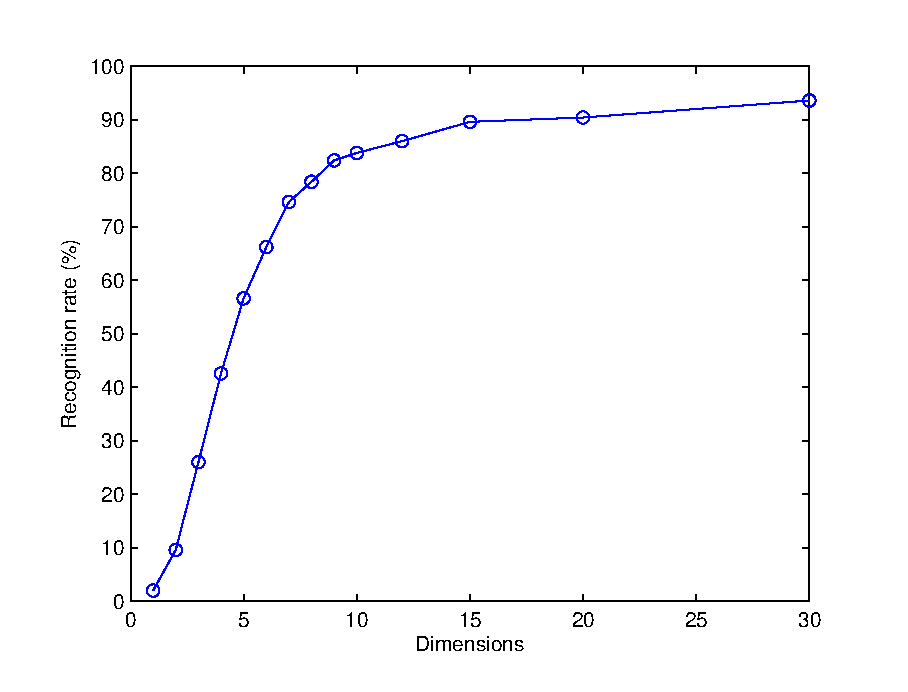
\includegraphics[width=\linewidth]{ch-experiment/figures/gamma}
    \caption[Recognition rate by OLDA for different dimensions]{Recognition rate by OLDA for different dimensions}
    \label{fig:experiment:gamma}
  \end{center}
\end{figure}

According to the curve shown in Figure ~\ref{fig:experiment:gamma}, $\Gamma=15$ is a good choice for the following experiments with balanced recognition rate and computation.
%!TEX root = chapter-experiment.tex
\section{Genuine and Imposter Distributions}
\label{sec:experiment:distribution}

Figure ~\ref{fig:experiment:11p} show the genuine and impostor distributions when the 15-dimensional features are applied to the 4000 training database when calculate the Euclidian distance.

\begin{figure}[htb]
  \begin{center}
    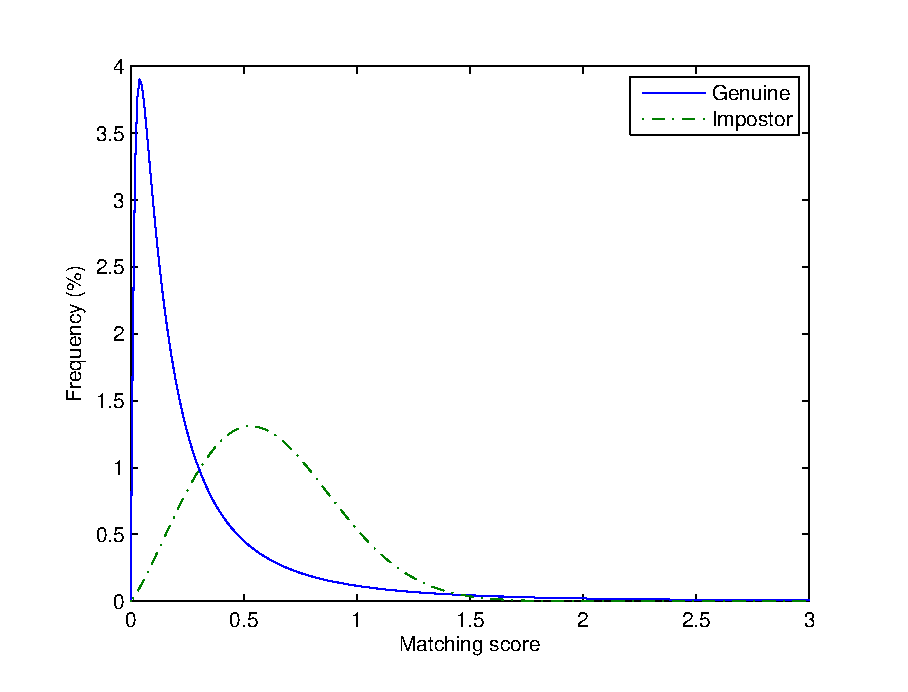
\includegraphics[scale=1]{ch-experiment/figures/11p.eps}
    \caption{Sample distributions by matching the 15-dimensional feature vector}
    \label{fig:experiment:11p}
  \end{center}
\end{figure}


%!TEX root = chapter-experiment.tex
\section{Recognition Performance}
\label{sec:experiment:recognition}

We next carried out the 3D palmprint classification and recognition experiments using the first sample of each class in the training database as a template and the 4000 samples in the testing database as probes, making a total of 400 templates and 4000 probes. The performance of classification and recognition is usually measured by error rate and penetration rate calculated in ~\cite{Maltoni:wn} as follows

\begin{equation}
\text{error rate} = \frac{\text{number of false match}}{\text{total number of probe}} \times 100\%
\end{equation}

\begin{equation}
\text{penetration rate} = \frac{\text{number of accessed template}}{\text{total number of template in the database}} \times 100\%
\label{eq:experiment:prate}
\end{equation}

Obviously there is a trade-off between error rates and penetration rates. Generally speaking, if there is no classification, there are two retrieval strategies:

\begin{enumerate}
\item all of the templates in the database are visited and the template that gives the best matching score is regarded as the matched template, if the matching score is less than a given threshold $\Psi_T$
\item given a threshold $\Psi_T$, the search continues until a match is found that is below that threshold
\end{enumerate}

Three 3D palmprint recognition matching approaches are used

\begin{enumerate}
\item no classification
\item coarse-level matching
\item RSVM
\end{enumerate}

For no classification, we matched using the local feature MCI as described in ~\cite{Zhang:2009dp}. The process we used for coarse-level matching is illustrated in Section ~\ref{sec:methodology:featurematch} and involves fine-level matching using the local feature MCI. A single instance of coarse-level matching requires only $1/36000$ of the time it takes to do fine-level matching (coarse-level matching only needs 15 operations while fine-level matching must do $128\times128\times(8\times4+1)$ operations, where $128\times128$ is the size of ROI and $8\times4+1$ is the number of times the template is shifted plus the original unshifted case). For the above two approaches, the penetration rate and the error rate will vary with different thresholds $\Psi_t$. As for RSVM, we use the RSVM algorithm described in Section ~\ref{ssec:methodology:svm} to rank the templates in the database, and then match the top $\rho$ percent by local feature MCI with the best matching score regarded as the matched template if this score is less than a given constant threshold $\Psi_T$. We can see from ~\ref{eq:experiment:prate} that $\rho$ is equal to the penetration rate. Given different thresholds $\Psi_t$ and $\rho$, we carried out a series of 3D palmprint recognition experiments.

% Table generated by Excel2LaTeX from sheet 'Sheet1'
\begin{table}[htbp]
  \centering
  \caption{Penetration rate and error rate with no classification}
    \begin{tabular}{cc}
    \toprule
    Penetration rate (\%) & Error rate (\%) \\
    \midrule
    100  & 1.29 \\
    51.1  & 1.68 \\
    49.3  & 1.86 \\
    47.2  & 2.1 \\
    45.9  & 2.33 \\
    43.7  & 2.6 \\
    42.6  & 2.95 \\
    41.5  & 3.3 \\
    40.3  & 3.75 \\
    38.1  & 4.8 \\
    35.9  & 5.86 \\
    \bottomrule
    \end{tabular}%
  \label{tab:experiment:noclass}%
\end{table}%

% Table generated by Excel2LaTeX from sheet 'Sheet1'
\begin{table}[htbp]
  \centering
  \caption{Penetration rate and error rate using coarse-level matching}
    \begin{tabular}{|c|c|}
    \hline
    Penetration rate (\%) & Error rate (\%) \\
    \hline
    45.2  & 1.31 \\ \hline
    41.6  & 1.32 \\ \hline
    38.8  & 1.36 \\ \hline
    34.7  & 1.42 \\ \hline
    29.1  & 1.56 \\ \hline
    23.5  & 1.78 \\ \hline
    20.5  & 2.12 \\ \hline
    18.4  & 2.39 \\ \hline
    13.3  & 3.16 \\ \hline
    10.1  & 4.3 \\ \hline
    8.6   & 5.79 \\
    \hline
    \end{tabular}%
  \label{tab:experiment:coarse}%
\end{table}%

% Table generated by Excel2LaTeX from sheet 'Sheet1'
\begin{table}[htbp]
  \centering
  \caption{Penetration rate and error rate using RSVM}
    \begin{tabular}{|c|c|}
    \hline
    Penetration rate (\%) & Error rate (\%) \\
    \hline
    30    & 1.3 \\ \hline
    27.5  & 1.33 \\ \hline
    25    & 1.37 \\ \hline
    22.5  & 1.42 \\ \hline
    20    & 1.49 \\ \hline
    17.5  & 1.63 \\ \hline
    15    & 1.87 \\ \hline
    12.5  & 2.48 \\ \hline
    10    & 3.35 \\ \hline
    7.5   & 4.41 \\ \hline
    5     & 5.88 \\
    \hline
    \end{tabular}%
  \label{tab:experiment:svm}%
\end{table}%


Table ~\ref{tab:experiment:noclass}, ~\ref{tab:experiment:coarse} and ~\ref{tab:experiment:svm} difference in penetration rate and error rate using different recognition strategies. Even at an approximately equal error rate, the proposed coarse-level matching and RSVM approaches get a much lower penetration rate than the no classification approach. Obviously RSVM has the best performance but requires an additional off-line training process compared to coarse-level matching.

\begin{figure}[htb]
\begin{center}
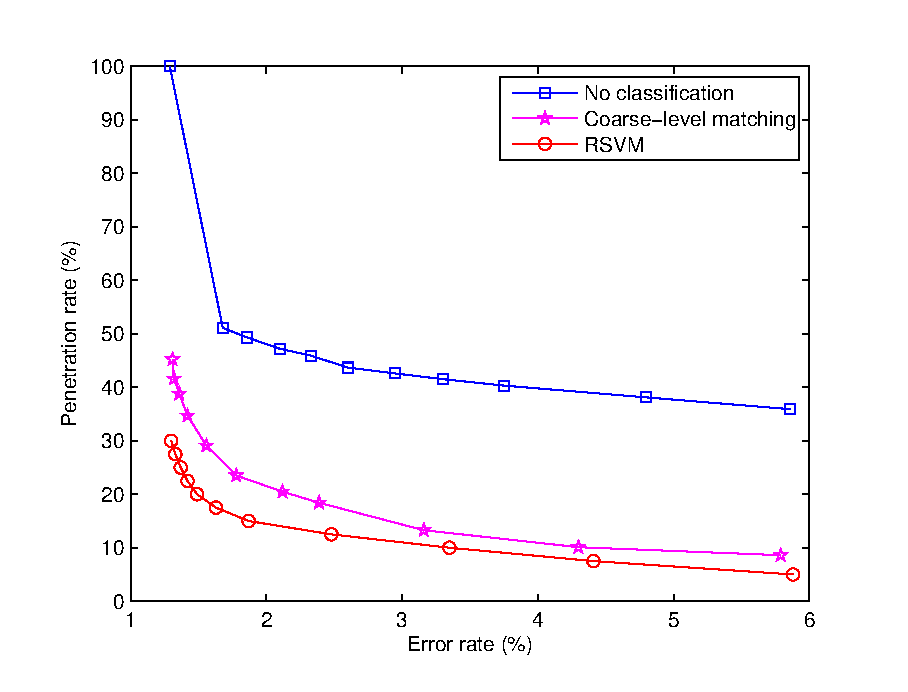
\includegraphics[width=\linewidth]{ch-experiment/figures/recognition}
\caption{Penetration rate and error rate with different matching strategies}
\label{fig:experiment:recognition}
\end{center}
\end{figure}

Figure ~\ref{fig:experiment:recognition} shows the results in a single plot.

% Table generated by Excel2LaTeX from sheet 'Sheet2'
\begin{table}[htbp]
  \centering
  \caption{Running time comparison of the three 3D palmprint recognition approaches}
    \begin{tabular}{lrrr}
    \toprule
          & No classification & Coarse-level matching & RSVM \\
    \midrule
    \multicolumn{1}{p{5cm}}{Once feature extraction time} & 112ms & 136ms & 136ms \\
    \multicolumn{1}{p{5cm}}{Once dimensionality reduction time} & 0ms   & 0.1ms & 0.1ms \\
    \multicolumn{1}{p{5cm}}{Ranking or coarse matching time for all templates in database} & 0ms   & 0.5ms & 1.56ms \\
    \multicolumn{1}{p{5cm}}{Once matching time by MCI} & 0.86ms & 0.86ms & 0.86ms \\
    \multicolumn{1}{p{5cm}}{Total running time for one probe testing} & 456ms & 292.09ms & 240.86ms \\
    \bottomrule
    \end{tabular}%
  \label{tab:experiment:time}%
\end{table}%



Table ~\ref{tab:experiment:time} shows the difference in time consumption for one probe. Due to the lower penetration rate, the running times are greatly reduced.

